\section{SSSP (Single Source Shortest Path)}
\subsection{Dijkstra}
\begin{frame}
\frametitle{Das Problem}
\begin{block}{Das Problem}
Breitensuche schlägt bei gewichteten Graphen fehl.
\end{block}
\end{frame}

\begin{frame}
\frametitle{Das Problem}
\begin{figure}
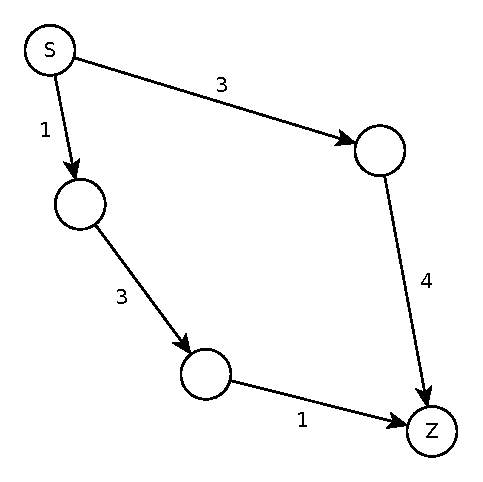
\includegraphics[scale=.8]{dijkstra_graphs/bfs_fail_0.pdf}
\end{figure}
\end{frame}

\begin{frame}
\frametitle{Das Problem}
\begin{figure}
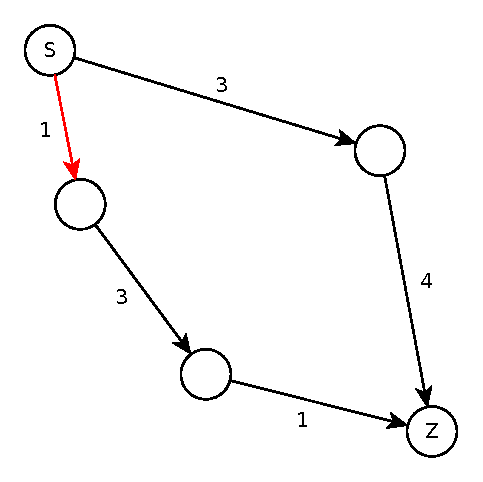
\includegraphics[scale=.8]{dijkstra_graphs/bfs_fail_1.pdf}
\end{figure}
\end{frame}

\begin{frame}
\frametitle{Das Problem}
\begin{figure}
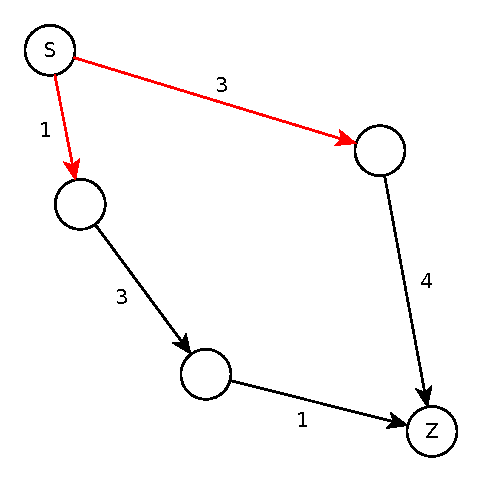
\includegraphics[scale=.8]{dijkstra_graphs/bfs_fail_2.pdf}
\end{figure}
\end{frame}

\begin{frame}
\frametitle{Das Problem}
\begin{figure}
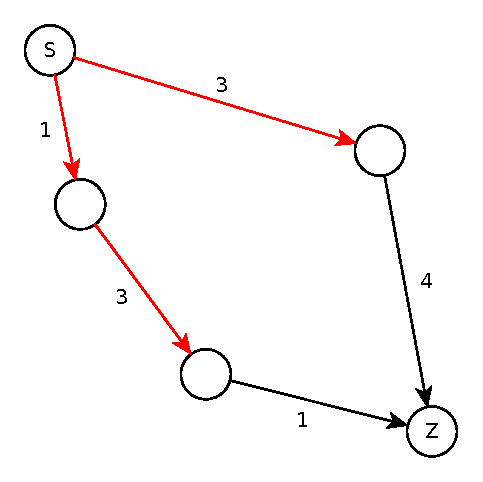
\includegraphics[scale=.8]{dijkstra_graphs/bfs_fail_3.pdf}
\end{figure}
\end{frame}

\begin{frame}
\frametitle{Das Problem}
\begin{figure}
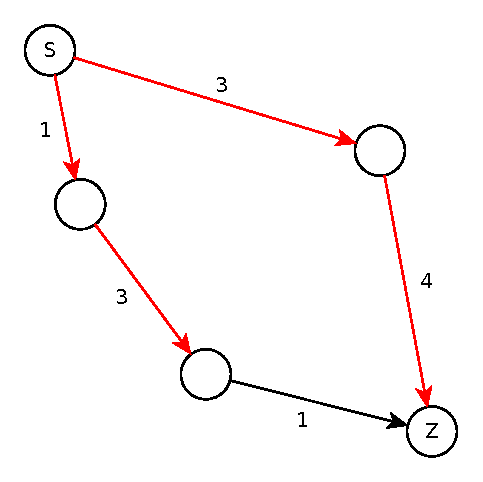
\includegraphics[scale=.8]{dijkstra_graphs/bfs_fail_4.pdf}
\end{figure}
\end{frame}

\begin{frame}
\frametitle{Das Problem}
\begin{figure}
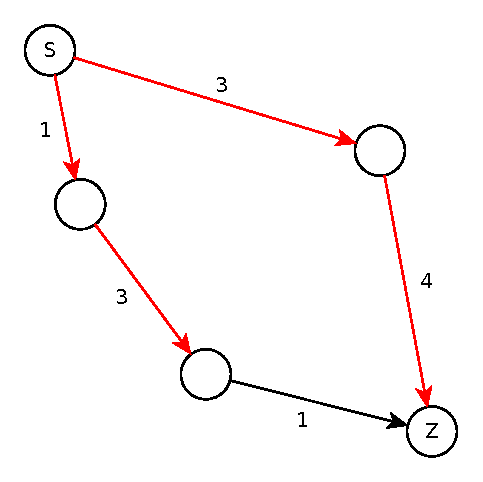
\includegraphics[scale=.8]{dijkstra_graphs/bfs_fail_4.pdf}
\end{figure}

$\implies$ Es wird ein Weg der Länge $7$ gefunden, obwohl $5$ das Optimum ist

\end{frame}


\begin{frame}
\frametitle{Djikstras Algorithmus}
\begin{itemize}
\item Grundsätzliche Idee: Breitensuche mit Priortiy-Queue (so dass "nähere" Knoten zuerst behandelt werden)
\item \lstinline|std::priority_queue| verwendet binären Heap
\item $\implies$ Laufzeit von Dijkstra ist $\Theta((n + m) \log n)$
\item Nachteil: Funktioniert nicht bei negativen Kantengewichten
\end{itemize}
\end{frame}

\begin{frame}[fragile]
\frametitle{Code}
Header: 
\begin{lstlisting}[basicstyle=\tiny]
#include<vector>
#include<algorithm>
#include<queue> // not priority_queue!
#include<iostream>

using namespace std;

struct arrival_event {
  int to;
  int weight;
};


bool operator < (const arrival_event& e1, const arrival_event& e2) {
	   // inversed
    return e1.weight > e2.weight;
}
\end{lstlisting}

\end{frame}

\begin{frame}[fragile]
\frametitle{Code}
\begin{lstlisting}[basicstyle=\tiny]
vector<int> dijkstra(vector<vector<arrival_event>>& nodes, int startnode) {
  vector<int> distances (nodes.size(), 2000000000);

  priority_queue<arrival_event> todo;

  todo.push({startnode, 0});

  while(!todo.empty()) {
    auto current = todo.top();
    todo.pop();

    if(current.weight < distances[current.to]) {
      distances[current.to] = current.weight;

      for(int i = 0; i < nodes[current.to].size(); i++) {
        arrival_event next = nodes[current.to][i];
        next.weight += current.weight;

        todo.push(next);
      }
    }
  }

  return distances;
}
\end{lstlisting}

\end{frame}


\begin{frame}
\frametitle{Beispiel}
\begin{figure}
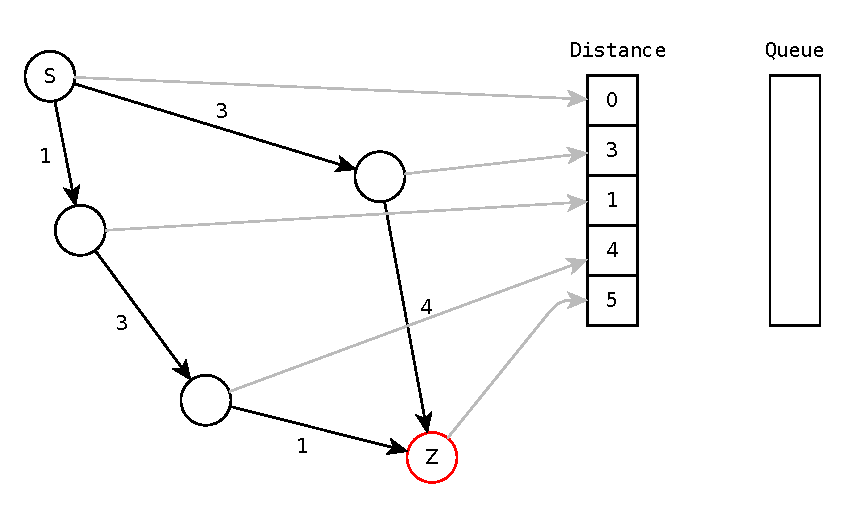
\includegraphics[scale=.8]{dijkstra_graphs/dijkstra_0.pdf}
\end{figure}
\end{frame}

\begin{frame}
\frametitle{Beispiel}
\begin{figure}
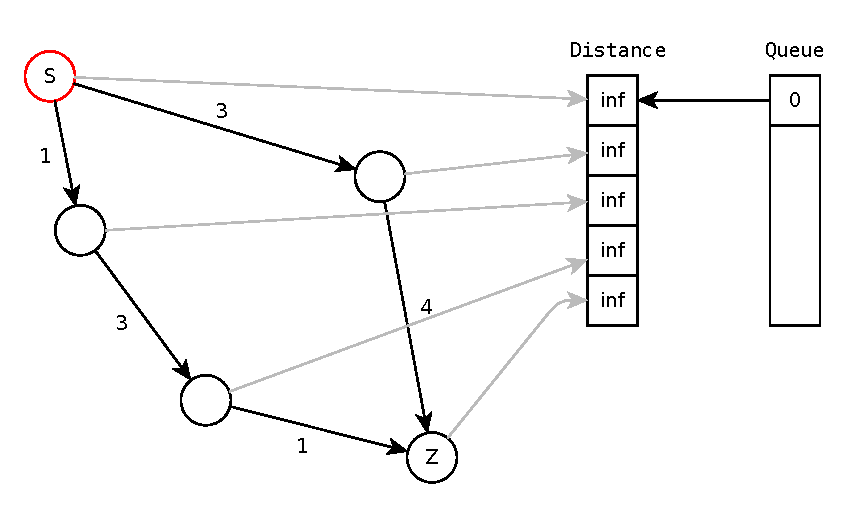
\includegraphics[scale=.8]{dijkstra_graphs/dijkstra_1.pdf}
\end{figure}
\end{frame}

\begin{frame}
\frametitle{Beispiel}
\begin{figure}
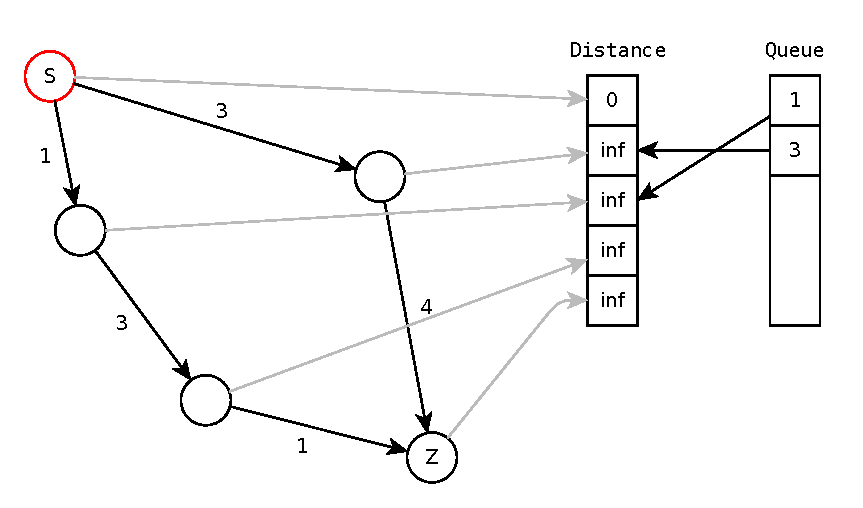
\includegraphics[scale=.8]{dijkstra_graphs/dijkstra_2.pdf}
\end{figure}
\end{frame}

\begin{frame}
\frametitle{Beispiel}
\begin{figure}
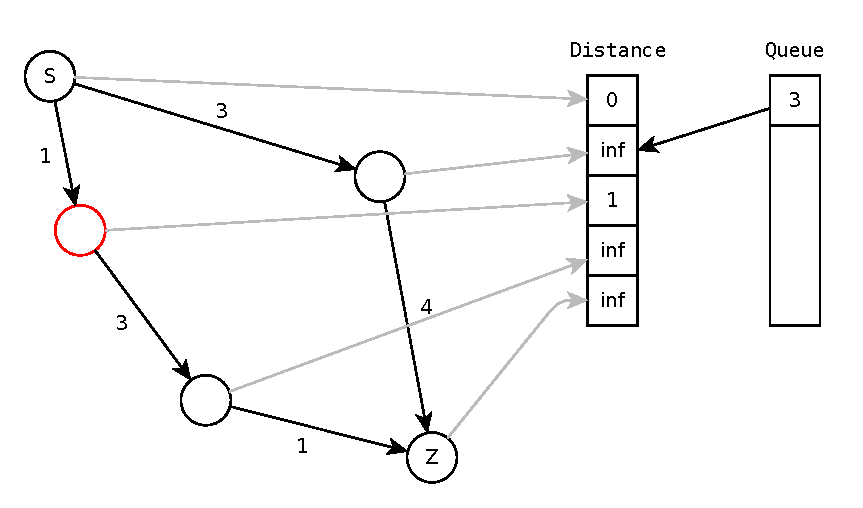
\includegraphics[scale=.8]{dijkstra_graphs/dijkstra_3.pdf}
\end{figure}
\end{frame}

\begin{frame}
\frametitle{Beispiel}
\begin{figure}
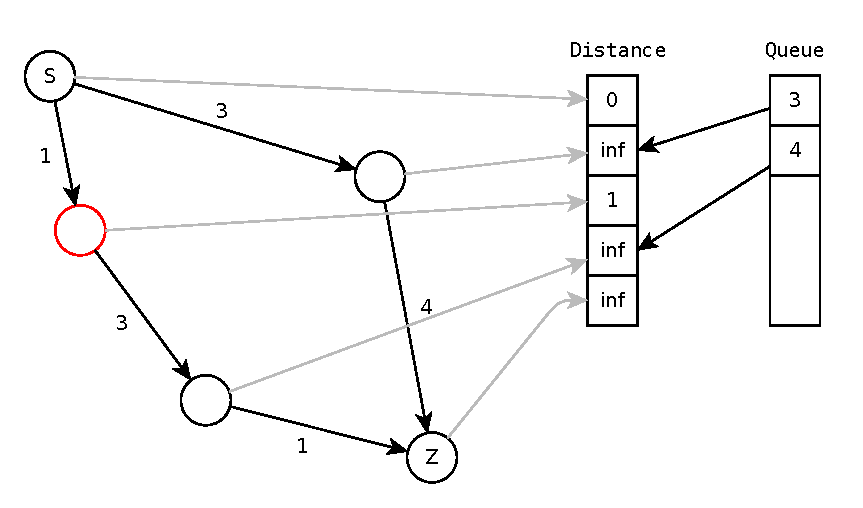
\includegraphics[scale=.8]{dijkstra_graphs/dijkstra_4.pdf}
\end{figure}
\end{frame}

\begin{frame}
\frametitle{Beispiel}
\begin{figure}
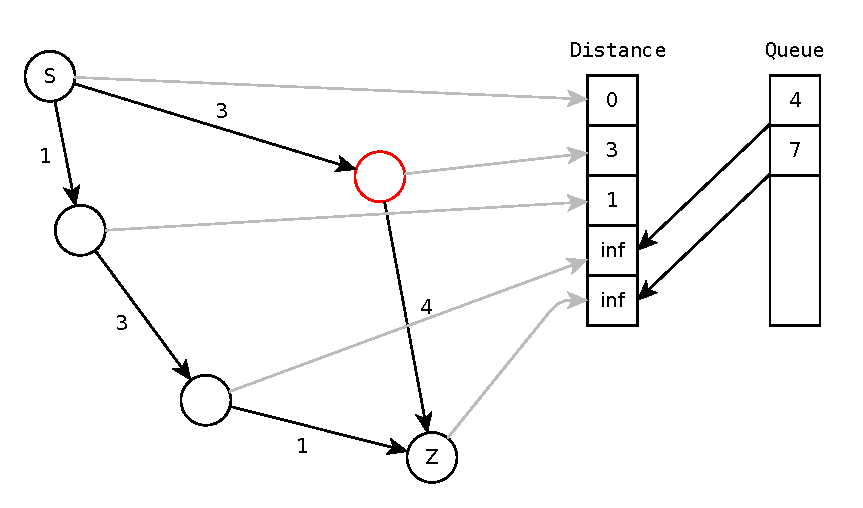
\includegraphics[scale=.8]{dijkstra_graphs/dijkstra_5.pdf}
\end{figure}
\end{frame}

\begin{frame}
\frametitle{Beispiel}
\begin{figure}
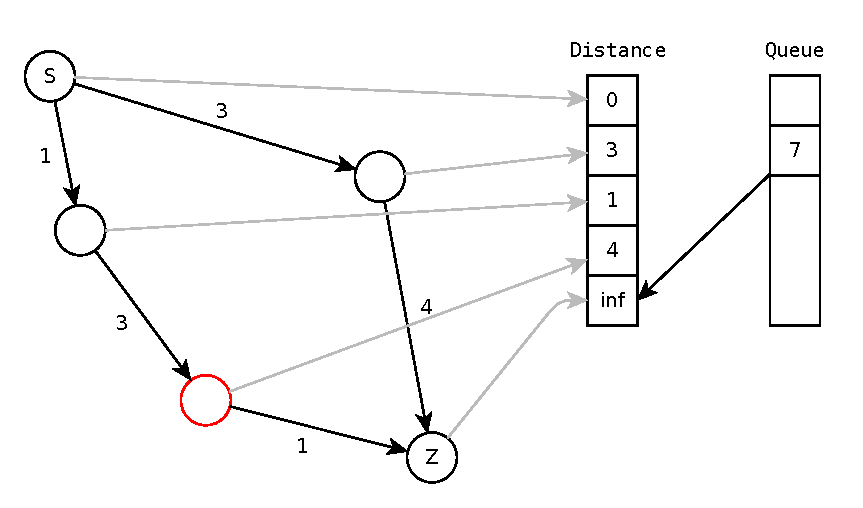
\includegraphics[scale=.8]{dijkstra_graphs/dijkstra_6.pdf}
\end{figure}
\end{frame}

\begin{frame}
\frametitle{Beispiel}
\begin{figure}
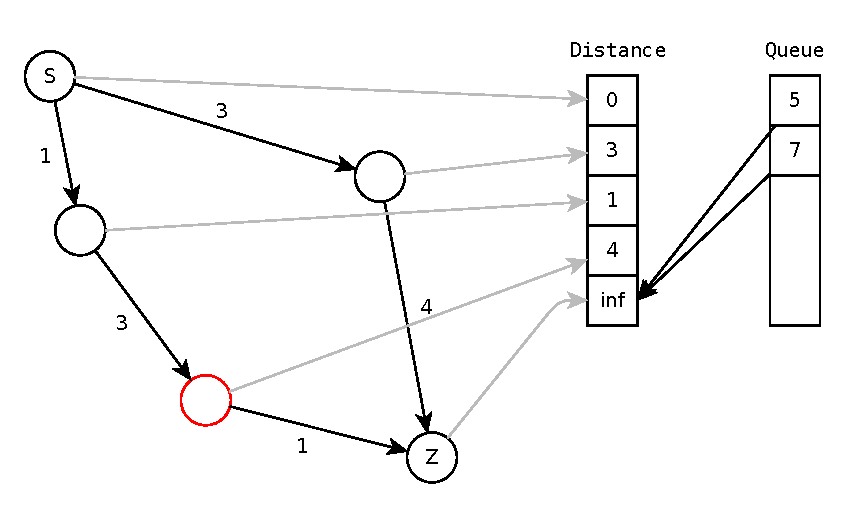
\includegraphics[scale=.8]{dijkstra_graphs/dijkstra_7.pdf}
\end{figure}
\end{frame}

\begin{frame}
\frametitle{Beispiel}
\begin{figure}
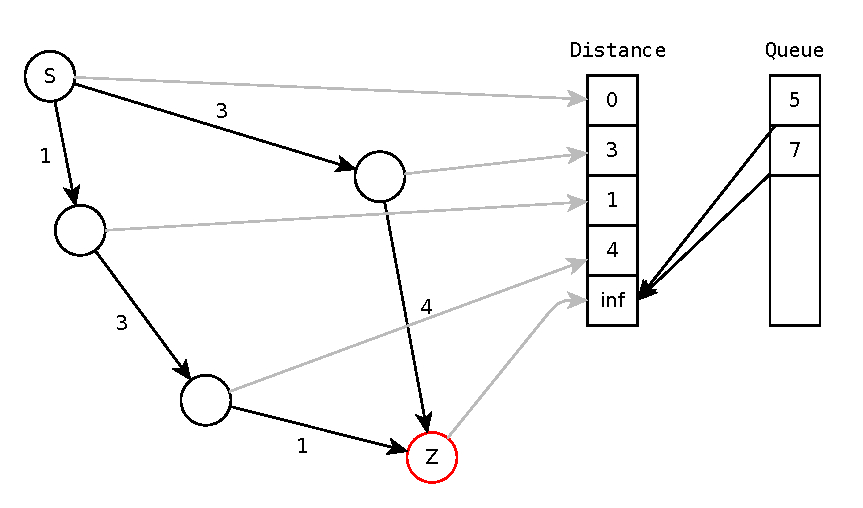
\includegraphics[scale=.8]{dijkstra_graphs/dijkstra_8.pdf}
\end{figure}
\end{frame}

\begin{frame}
\frametitle{Beispiel}
\begin{figure}
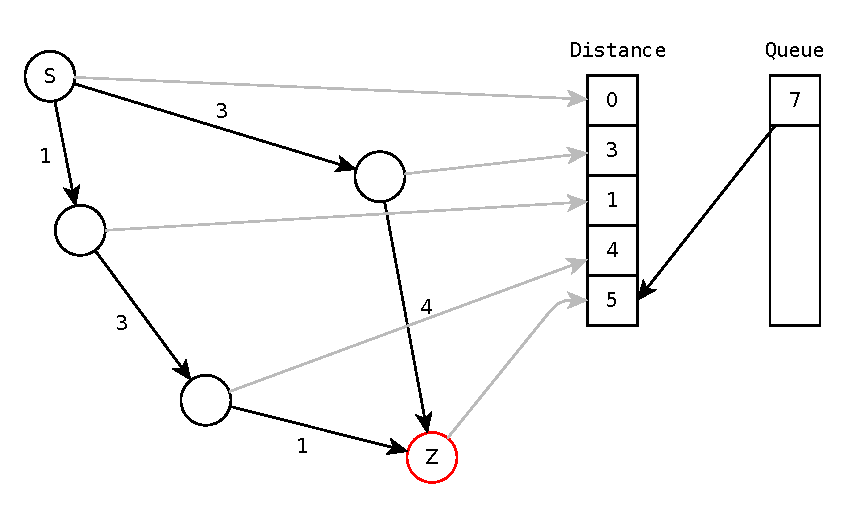
\includegraphics[scale=.8]{dijkstra_graphs/dijkstra_9.pdf}
\end{figure}
\end{frame}

\begin{frame}
\frametitle{Beispiel}
\begin{figure}
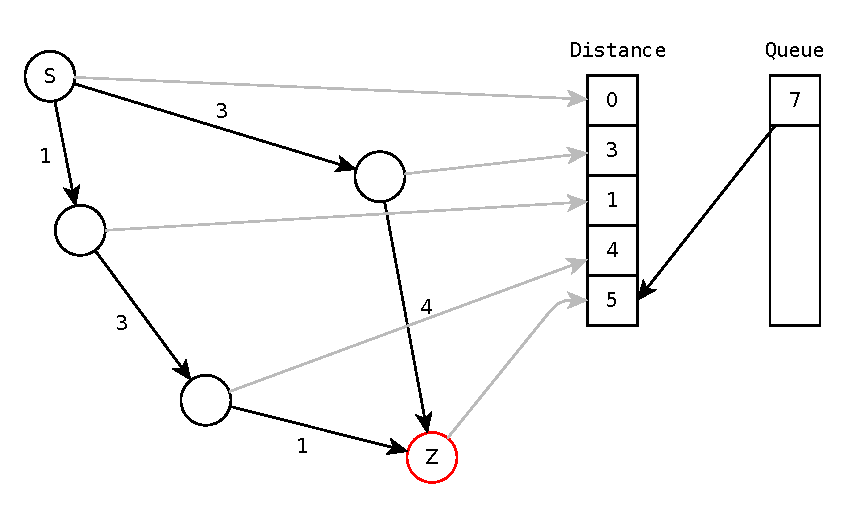
\includegraphics[scale=.8]{dijkstra_graphs/dijkstra_A.pdf}
\end{figure}
\end{frame}

\begin{frame}
\frametitle{Beispiel}
\begin{figure}
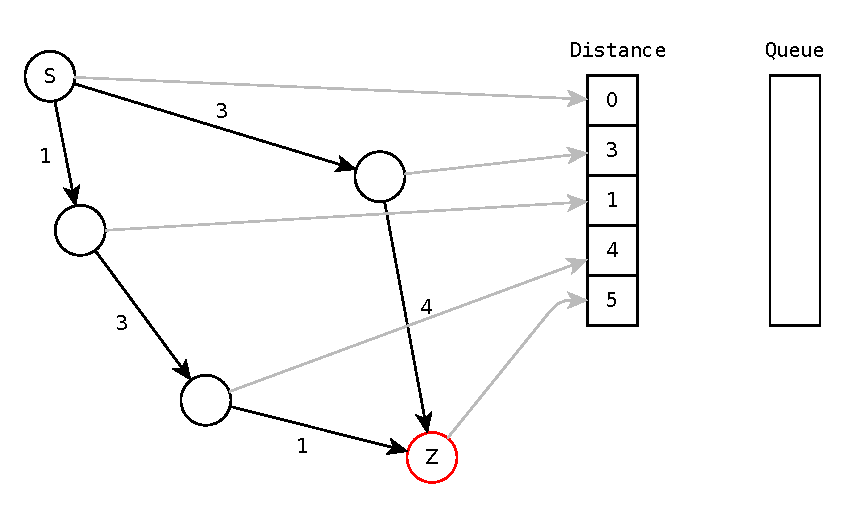
\includegraphics[scale=.8]{dijkstra_graphs/dijkstra_B.pdf}
\end{figure}
\end{frame}